\section{Register description}
\regover{
{\hyperref[emac-MODE]{MODE}}&EMAC configuration
\\
\hline
{\hyperref[emac-INT-SOURCE]{INT\_SOURCE}}&EMAC transmit control
\\
\hline
{\hyperref[emac-INT-MASK]{INT\_MASK}}&EMAC interrupt mask
\\
\hline
{\hyperref[emac-IPGT]{IPGT}}&Inter packet gap
\\
\hline
{\hyperref[emac-PACKETLEN]{PACKETLEN}}&Frame length
\\
\hline
{\hyperref[emac-COLLCONFIG]{COLLCONFIG}}&Collision configuration
\\
\hline
{\hyperref[emac-TX-BD-NUM]{TX\_BD\_NUM}}&TX buffer descriptors number
\\
\hline
{\hyperref[emac-MIIMODE]{MIIMODE}}&Management Data configuration
\\
\hline
{\hyperref[emac-MIICOMMAND]{MIICOMMAND}}&Trigger command
\\
\hline
{\hyperref[emac-MIIADDRESS]{MIIADDRESS}}&Register address
\\
\hline
{\hyperref[emac-MIITX-DATA]{MIITX\_DATA}}&Control data to be written to PHY
\\
\hline
{\hyperref[emac-MIIRX-DATA]{MIIRX\_DATA}}&Received data from PHY
\\
\hline
{\hyperref[emac-MIISTATUS]{MIISTATUS}}&MIIM I/F status
\\
\hline
{\hyperref[emac-MAC-ADDR0]{MAC\_ADDR0}}&Ethernet MAC address0
\\
\hline
{\hyperref[emac-MAC-ADDR1]{MAC\_ADDR1}}&Ethernet MAC address1
\\
\hline
{\hyperref[emac-HASH0-ADDR]{HASH0\_ADDR}}&Lower 32-bit of HASH register
\\
\hline
{\hyperref[emac-HASH1-ADDR]{HASH1\_ADDR}}&Upper 32-bit of HASH register
\\
\hline
{\hyperref[emac-TXCTRL]{TXCTRL}}&TX control
\\
\hline
}

\subsection{MODE}
\label{emac-MODE}
Address:0x4000d000
 \begin{figure}[H]
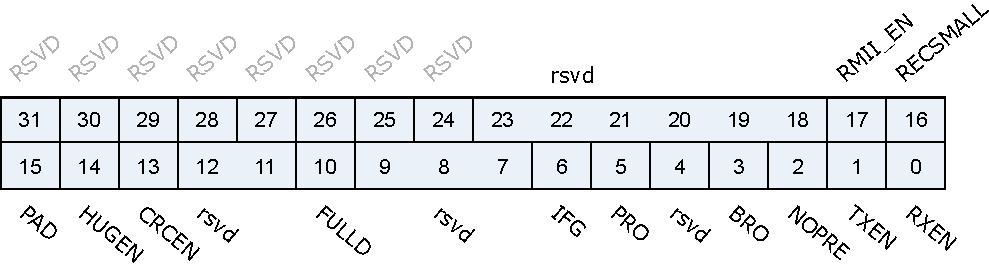
\includegraphics{emac_MODE.pdf}
\end{figure}

\regdes{31:18&RSVD& & & \\\hline
17&RMII\_EN&r/w&1'b0&RMII mode enable \par 0: MII PHY I/F is used \par 1: RMII PHY I/F is used
\\\hline
16&RECSMALL&r/w&1'b0&Receive small frame enable \par 0: Frames smaller than MINFL are ignored. \par 1: Frames smaller than MINFL are accepted.
\\\hline
15&PAD&r/w&1'b1&Padding enable \par 0: Do not add pads to frames shorter than MINFL. \par 1: Add pads to short frames, until the length equals MINFL.
\\\hline
14&HUGEN&r/w&1'b0&Huge frames enable \par 0: The maximum frame length is MAXFL. All additional bytes are dropped. \par 1: Frame size is not limited by MAXFL and can be up to 64K bytes.
\\\hline
13&CRCEN&r/w&1'b1&CRC Enable \par 0: TX MAC does not append CRC field. \par 1: TX MAC will append CRC field to every frame.
\\\hline
12:11&RSVD& & & \\\hline
10&FULLD&r/w&1'b0&Full duplex \par 0: Half duplex mode. \par 1: Full duplex mode.
\\\hline
9:7&RSVD& & & \\\hline
6&IFG&r/w&1'b0&Inter frame gap check \par 0: IFG is verified before each frame be received. \par 1: All frames are received regardless to IFG requirement.
\\\hline
5&PRO&r/w&1'b0&Promiscuous mode enable \par 0: The destination address is checked before receiving. \par 1: All frames received regardless of the address.
\\\hline
4&RSVD& & & \\\hline
3&BRO&r/w&1'b1&Broadcast address enable \par 0: Reject all frames containing the broadcast address unless the PRO bit is asserted. \par 1: Receive all frames containing broadcast address.
\\\hline
2&NOPRE&r/w&1'b0&No preamble mode \par 0: 7-byte preamble will be sent. \par 1: No preamble will be sent.
\\\hline
1&TXEN&r/w&1'b0&Transmit enable \par 0: Transmitter is disabled. \par 1: Transmitter is enabled. \par If TX\_BD\_NUM equals 0x0 (zero buffer descriptors are used), then the transmitter is disabled regardless of TXEN.
\\\hline
0&RXEN&r/w&1'b0&Receiver enable \par 0: Receiver is disabled. \par 1: Receiver is enabled. \par If TX\_BD\_NUM equals 0x80 (all buffer descriptors are used for TX), then the receiver is disabled regardless of RXEN.
\\\hline

}
\subsection{INT\_SOURCE}
\label{emac-INT-SOURCE}
Address:0x4000d004
 \begin{figure}[H]
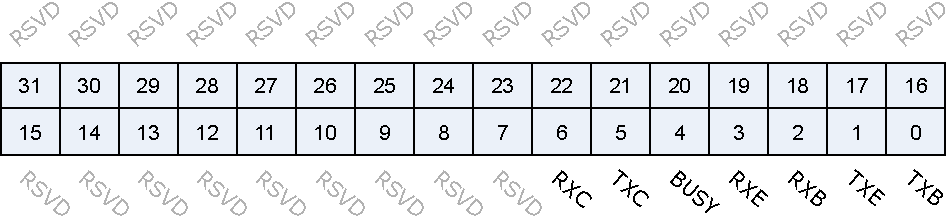
\includegraphics{emac_INT_SOURCE.pdf}
\end{figure}

\regdes{31:7&RSVD& & & \\\hline
6&RXC&r/w&1'b0&Receive control frame \par This bit indicates that the control frame was received. It is cleared by writing 1 to it. \par Bit RXFLOW in the CTRLMODE register must be set to 1 in order to get the RXC bit set.
\\\hline
5&TXC&r/w&1'b0&Transmit control frame \par This bit indicates that a control frame was transmitted. It is cleared by writing 1 to it. \par Bit TXFLOW in the CTRLMODE register must be set to 1 in order to get the TXC bit set.
\\\hline
4&BUSY&r/w&1'b0&Busy \par This bit indicates that RX packet is being received and there is no empty buffer descriptor to use. It iscleared by writing 1 to it. \par This bit appears regardless to the IRQ bits in the Receive Buffer Descriptor.
\\\hline
3&RXE&r/w&1'b0&Receive error \par This bit indicates that an error occurred while receiving data (overrun, receiver error, dribble \par nibble, too long, >64K, CRC error, bus error or late collision. It is cleared by writing 1 to it. \par This bit appears only when IRQ bit is set in the Receive Buffer Descriptor.
\\\hline
2&RXB&r/w&1'b0&Receive frame \par This bit indicates that a frame was received. It is cleared by writing 1 to it. \par This bit appears only when IRQ bit is set in the Receive Buffer Descriptor.
\\\hline
1&TXE&r/w&1'b0&Transmit error \par This bit indicates that a buffer was not transmitted due to a transmit error (underrun, \par retransmission limit, late collision, bus error or defer timeout). It is cleared by writing 1 to it. \par This bit appears only when IRQ bit is set in the Transmit Buffer Descriptor.
\\\hline
0&TXB&r/w&1'b0&Transmit buffer \par This bit indicates that a buffer has been transmitted. It is cleared by writing 1 to it. \par This bit appears only when IRQ bit is set in the Transmit Buffer Descriptor.
\\\hline

}
\subsection{INT\_MASK}
\label{emac-INT-MASK}
Address:0x4000d008
 \begin{figure}[H]
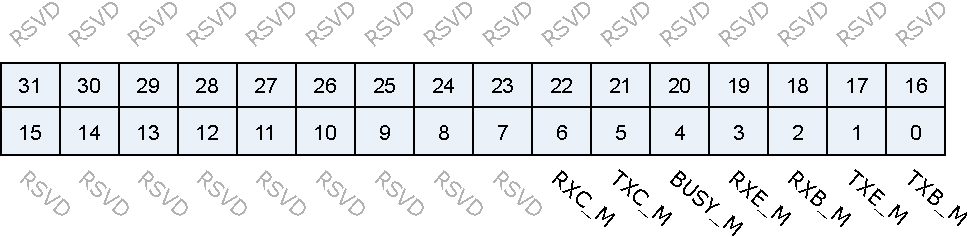
\includegraphics{emac_INT_MASK.pdf}
\end{figure}

\regdes{31:7&RSVD& & & \\\hline
6&RXC\_M&r/w&1'b1&Receive control frame mask ENABLE \par 0: Interrupt is un-masked \par 1: Interrupt is masked
\\\hline
5&TXC\_M&r/w&1'b1&Transmit control frame mask ENABLE \par 0: Interrupt is un-masked \par 1: Interrupt is masked
\\\hline
4&BUSY\_M&r/w&1'b1&Busy mask ENABLE \par 0: Interrupt is un-masked \par 1: Interrupt is masked
\\\hline
3&RXE\_M&r/w&1'b1&Receive error mask ENABLE \par 0: Interrupt is un-masked \par 1: Interrupt is masked
\\\hline
2&RXB\_M&r/w&1'b1&Receive frame mask ENABLE \par 0: Interrupt is un-masked \par 1: Interrupt is masked
\\\hline
1&TXE\_M&r/w&1'b1&Transmit error mask ENABLE \par 0: Interrupt is un-masked \par 1: Interrupt is masked
\\\hline
0&TXB\_M&r/w&1'b1&Transmit buffer mask ENABLE \par 0: Interrupt is un-masked \par 1: Interrupt is masked
\\\hline

}
\subsection{IPGT}
\label{emac-IPGT}
Address:0x4000d00c
 \begin{figure}[H]
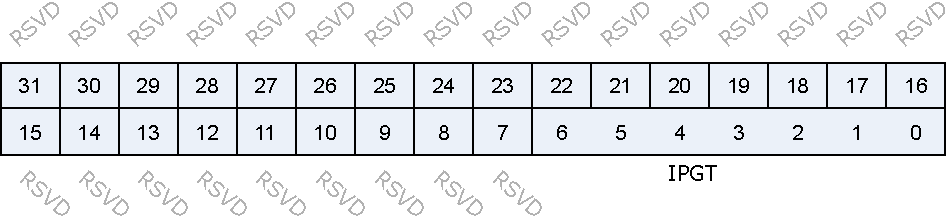
\includegraphics{emac_IPGT.pdf}
\end{figure}

\regdes{31:7&RSVD& & & \\\hline
6:0&IPGT&r/w&7'h18&Inter packet gap \par The recommended value is 0x18 (24 clock cycles), \par which equals 9.6 us for 10 Mbps and 0.96 us for 100 Mbps mode
\\\hline

}
\subsection{PACKETLEN}
\label{emac-PACKETLEN}
Address:0x4000d018
 \begin{figure}[H]
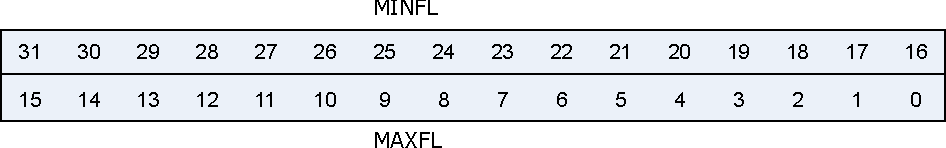
\includegraphics{emac_PACKETLEN.pdf}
\end{figure}

\regdes{31:16&MINFL&r/w&16'h40&Minimum frame length \par The minimum Ethernet packet is 64 bytes long (0x40). \par To receive small packets, assert the RECSMALL bit or change the MINFL value. \par To transmit small packets, assert the PAD bit or change the MINFL value.
\\\hline
15:0&MAXFL&r/w&16'h600&Maximum frame length \par The maximum Ethernet packet is 1518 bytes long. To support this and to have some additional \par space for tags, a default maximum packet length equals to 1536 bytes (0x600). \par For bigger packets, you can assert the HUGEN bit or increase the value of MAXFL field.
\\\hline

}
\subsection{COLLCONFIG}
\label{emac-COLLCONFIG}
Address:0x4000d01c
 \begin{figure}[H]
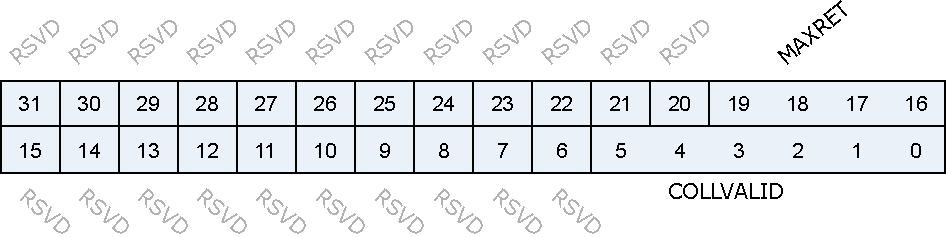
\includegraphics{emac_COLLCONFIG.pdf}
\end{figure}

\regdes{31:20&RSVD& & & \\\hline
19:16&MAXRET&r/w&4'hF&Maximum retry \par This field specifies the maximum number of consequential retransmission attempts after the collision is detected. \par When the maximum number has been reached, the TX MAC reports an error and stops transmitting the current packet. \par According to the Ethernet standard, the MAXRET default value is set to 0xf (15).
\\\hline
15:6&RSVD& & & \\\hline
5:0&COLLVALID&r/w&6'h3F&Collision valid \par This field specifies a collision time window. A collision that occurs later than the time window \par is reported as a "Late Collisions" and transmission of the current packet is aborted.
\\\hline

}
\subsection{TX\_BD\_NUM}
\label{emac-TX-BD-NUM}
Address:0x4000d020
 \begin{figure}[H]
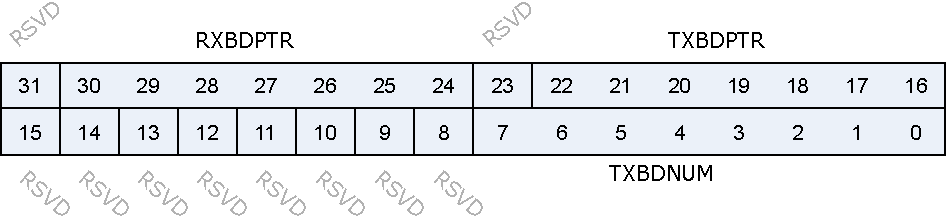
\includegraphics{emac_TX_BD_NUM.pdf}
\end{figure}

\regdes{31&RSVD& & & \\\hline
30:24&RXBDPTR&r&7'h0&RX buffer descriptors (BD) pointer, pointing at the RXBD currently being used\\\hline
23&RSVD& & & \\\hline
22:16&TXBDPTR&r&7'h0&TX buffer descriptors (BD) pointer, pointing at the TXBD currently being used\\\hline
15:8&RSVD& & & \\\hline
7:0&TXBDNUM&r/w&8'h40&TX buffer descriptors (BD) number \par Number of TX BD. TX and RX share 128 (0x80) descriptors, so the number of RX BD equals 0x80 - TXBDNUM. \par The maximum number of TXBDNUM is 0x80. Values greater then 0x80 cannot be written into this register.
\\\hline

}
\subsection{MIIMODE}
\label{emac-MIIMODE}
Address:0x4000d028
 \begin{figure}[H]
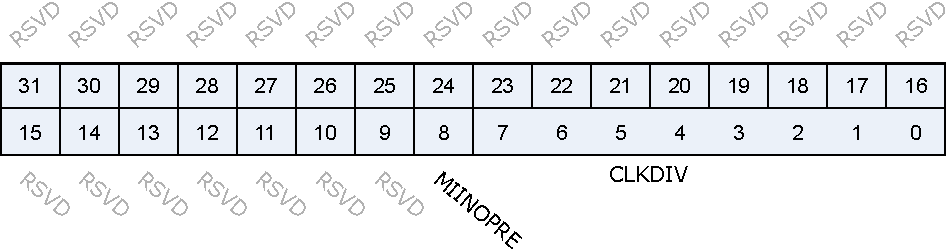
\includegraphics{emac_MIIMODE.pdf}
\end{figure}

\regdes{31:9&RSVD& & & \\\hline
8&MIINOPRE&r/w&1'b0&No preamble for Management Data (MD) \par 0: 32-bit preamble will be sent. \par 1: No preamble will be sent.
\\\hline
7:0&CLKDIV&r/w&8'h64&Clock divider for Management Data Clock (MDC) \par The source clock is bus clock and can be divided by any even number.
\\\hline

}
\subsection{MIICOMMAND}
\label{emac-MIICOMMAND}
Address:0x4000d02c
 \begin{figure}[H]
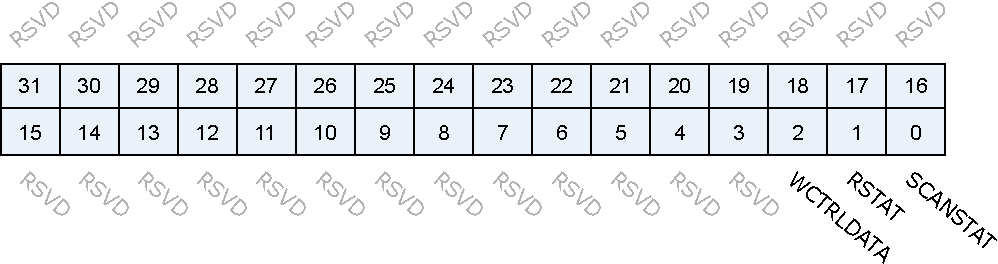
\includegraphics{emac_MIICOMMAND.pdf}
\end{figure}

\regdes{31:3&RSVD& & & \\\hline
2&WCTRLDATA&r/w&1'b0&Write control data, setting this bit to 1 will trigger the command (auto cleared) \par Note: [2]/[1]/[0] cannot be asserted at the same time, execute one command at a time
\\\hline
1&RSTAT&r/w&1'b0&Read status, setting this bit to 1 will trigger the command (auto cleared) \par Note: [2]/[1]/[0] cannot be asserted at the same time, execute one command at a time
\\\hline
0&SCANSTAT&r/w&1'b0&Scan status, setting this bit to 1 will trigger the command (auto cleared) \par Note: [2]/[1]/[0] cannot be asserted at the same time, execute one command at a time
\\\hline

}
\subsection{MIIADDRESS}
\label{emac-MIIADDRESS}
Address:0x4000d030
 \begin{figure}[H]
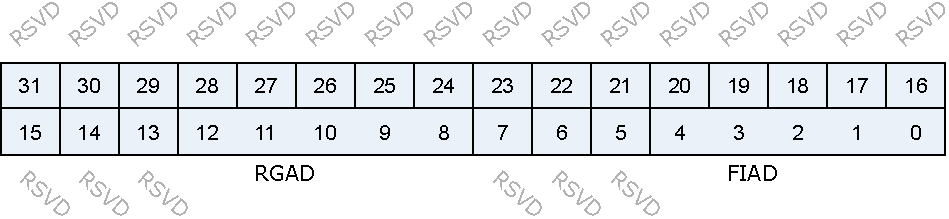
\includegraphics{emac_MIIADDRESS.pdf}
\end{figure}

\regdes{31:13&RSVD& & & \\\hline
12:8&RGAD&r/w&5'h0&Register Address\\\hline
7:5&RSVD& & & \\\hline
4:0&FIAD&r/w&5'h0&PHY Address\\\hline

}
\subsection{MIITX\_DATA}
\label{emac-MIITX-DATA}
Address:0x4000d034
 \begin{figure}[H]
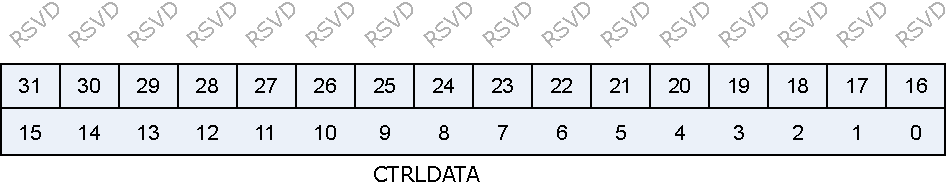
\includegraphics{emac_MIITX_DATA.pdf}
\end{figure}

\regdes{31:16&RSVD& & & \\\hline
15:0&CTRLDATA&r/w&16'h0&Control Data to be written to PHY\\\hline

}
\subsection{MIIRX\_DATA}
\label{emac-MIIRX-DATA}
Address:0x4000d038
 \begin{figure}[H]
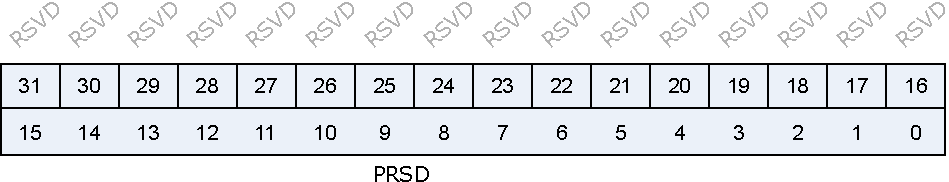
\includegraphics{emac_MIIRX_DATA.pdf}
\end{figure}

\regdes{31:16&RSVD& & & \\\hline
15:0&PRSD&r&16'h0&Received Data from PHY\\\hline

}
\subsection{MIISTATUS}
\label{emac-MIISTATUS}
Address:0x4000d03c
 \begin{figure}[H]
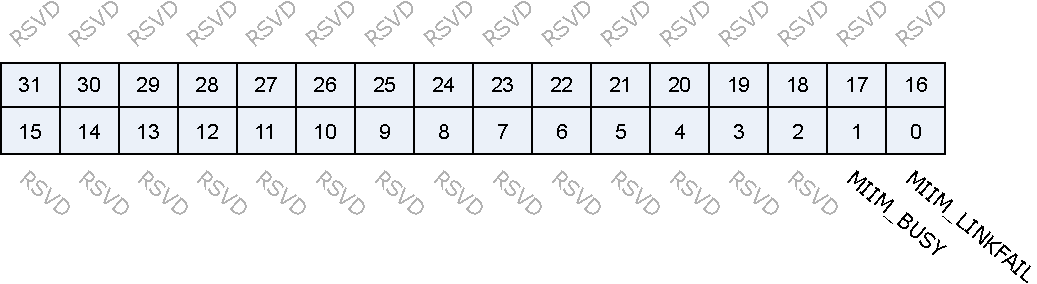
\includegraphics{emac_MIISTATUS.pdf}
\end{figure}

\regdes{31:2&RSVD& & & \\\hline
1&MIIM\_BUSY&r&1'b0&MIIM I/F busy signal \par 0: The MIIM I/F is ready. \par 1: The MIIM I/F is busy.
\\\hline
0&MIIM\_LINKFAIL&r&1'b0&MIIM I/F link fail signal\\\hline

}
\subsection{MAC\_ADDR0}
\label{emac-MAC-ADDR0}
Address:0x4000d040
 \begin{figure}[H]
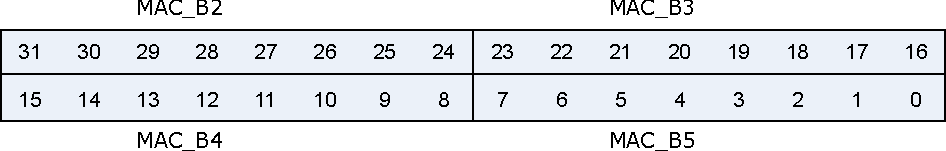
\includegraphics{emac_MAC_ADDR0.pdf}
\end{figure}

\regdes{31:24&MAC\_B2&r/w&8'd0&Ethernet MAC address byte 2\\\hline
23:16&MAC\_B3&r/w&8'd0&Ethernet MAC address byte 3\\\hline
15:8&MAC\_B4&r/w&8'd0&Ethernet MAC address byte 4\\\hline
7:0&MAC\_B5&r/w&8'd0&Ethernet MAC address byte 5\\\hline

}
\subsection{MAC\_ADDR1}
\label{emac-MAC-ADDR1}
Address:0x4000d044
 \begin{figure}[H]
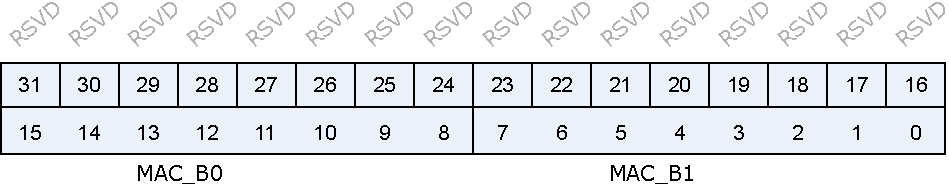
\includegraphics{emac_MAC_ADDR1.pdf}
\end{figure}

\regdes{31:16&RSVD& & & \\\hline
15:8&MAC\_B0&r/w&8'd0&Ethernet MAC address byte 0\\\hline
7:0&MAC\_B1&r/w&8'd0&Ethernet MAC address byte 1\\\hline

}
\subsection{HASH0\_ADDR}
\label{emac-HASH0-ADDR}
Address:0x4000d048
 \begin{figure}[H]
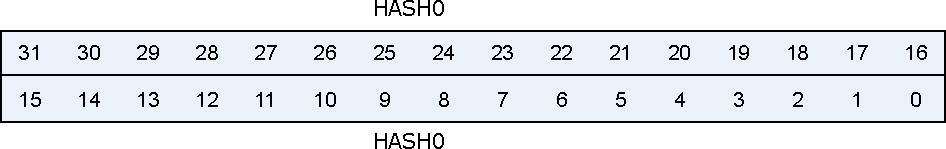
\includegraphics{emac_HASH0_ADDR.pdf}
\end{figure}

\regdes{31:0&HASH0&r/w&32'h0&Lower 32-bit of HASH register\\\hline

}
\subsection{HASH1\_ADDR}
\label{emac-HASH1-ADDR}
Address:0x4000d04c
 \begin{figure}[H]
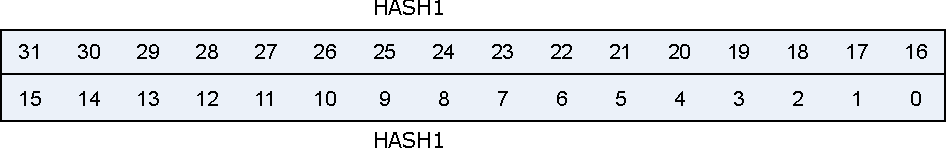
\includegraphics{emac_HASH1_ADDR.pdf}
\end{figure}

\regdes{31:0&HASH1&r/w&32'h0&Upper 32-bit of HASH register\\\hline

}
\subsection{TXCTRL}
\label{emac-TXCTRL}
Address:0x4000d050
 \begin{figure}[H]
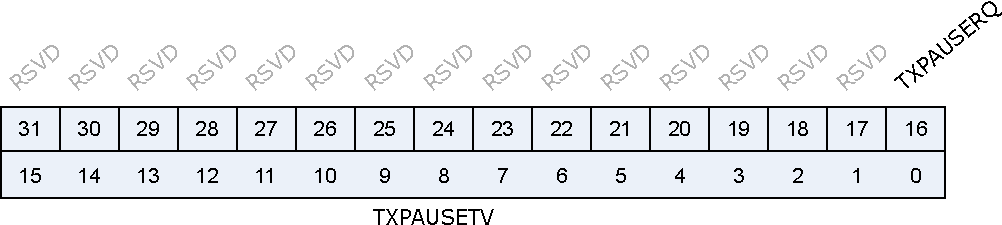
\includegraphics{emac_TXCTRL.pdf}
\end{figure}

\regdes{31:17&RSVD& & & \\\hline
16&TXPAUSERQ&r/w&1'b0&TX Pause Request \par Writing 1 to this bit starts sending control frame and is automatically cleared to zero.
\\\hline
15:0&TXPAUSETV&r/w&16'h0&TX Pause Timer Value \par The value that is sent in the pause control frame.
\\\hline

}
